\documentclass[twocolumn, amsmath, amsfonts, amssymb]{aastex62}
\usepackage{mathtools}
\usepackage{natbib}
\usepackage{bm}
\newcommand{\vdag}{(v)^\dagger}
\newcommand\aastex{AAS\TeX}
\newcommand\latex{La\TeX}


\newcommand{\Div}[1]{\ensuremath{\nabla\cdot\left( #1\right)}}
\newcommand{\DivU}{\ensuremath{\nabla\cdot\bm{u}}}
\newcommand{\angles}[1]{\ensuremath{\left\langle #1 \right\rangle}}
\newcommand{\KS}[1]{\ensuremath{\text{KS}(#1)}}
\newcommand{\KSstat}[1]{\ensuremath{\overline{\text{KS}(#1)}}}
\newcommand{\grad}{\ensuremath{\nabla}}
\newcommand{\RB}{Rayleigh-B\'{e}nard }
\newcommand{\stressT}{\ensuremath{\bm{\bar{\bar{\Pi}}}}}
\newcommand{\lilstressT}{\ensuremath{\bm{\bar{\bar{\sigma}}}}}
\newcommand{\nrho}{\ensuremath{n_{\rho}}}
\newcommand{\approptoinn}[2]{\mathrel{\vcenter{
	\offinterlineskip\halign{\hfil$##$\cr
	#1\propto\cr\noalign{\kern2pt}#1\sim\cr\noalign{\kern-2pt}}}}}

\newcommand{\appropto}{\mathpalette\approptoinn\relax}
\newcommand{\pro}{\ensuremath{\text{Ro}_{\text{p}}}}
\newcommand{\con}{\ensuremath{\text{Ro}_{\text{c}}}}

\usepackage{color}
\newcommand{\gv}[1]{{\color{blue} #1}}

%% Tells LaTeX to search for image files in the 
%% current directory as well as in the figures/ folder.
\graphicspath{{./}{figs/}}


\received{\today}
\revised{??}%\today}
\accepted{??}%\today}
\submitjournal{ApJL}

%%%%%%%%%%%%%%%%%%%%%%%%%%%%%%%%%%%%%%%%%%%%%%%%%%%%%%%%%%%%%%%%%%%%%%%%%%%%%%%
%% TITLE & AUTHORS
\shorttitle{Predicting the Rossby number in convective experiments}
\shortauthors{Anders et al.}

\begin{document}
\defcitealias{anders&brown2017}{AB17}
\newcommand{\AB}{\citetalias{anders&brown2017}}

\title{Predicting the Rossby number in convective experiments}

\correspondingauthor{Evan H. Anders}
\email{evan.anders@colorado.edu}

\author{Evan H. Anders}
\affil{Dept. Astrophysical \& Planetary Sciences, University of Colorado -- Boulder, Boulder, CO 80309, USA}
\affil{Laboratory for Atmospheric and Space Physics, Boulder, CO 80303, USA}
\author{Cathryn M. Manduca}
\affil{Laboratory for Atmospheric and Space Physics, Boulder, CO 80303, USA}
\author{Benjamin P. Brown}
\affil{Dept. Astrophysical \& Planetary Sciences, University of Colorado -- Boulder, Boulder, CO 80309, USA}
\affil{Laboratory for Atmospheric and Space Physics, Boulder, CO 80303, USA}
\author{Jeffrey S. Oishi}
\affiliation{Department of Physics and Astronomy, Bates College, Lewiston, ME 04240, USA}
\author{Geoffrey M. Vasil}
\affiliation{University of Sydney School of Mathematics and Statistics, Sydney, NSW 2006, Australia}


\begin{abstract}
  The Rossby number is a crucial parameter describing the degree of rotational constraint on the convective dynamics in stars and planets. 
However, it is not an input to computational models of convection but must be measured ex post facto. 
Here, we report the discovery of a new quantity, the Predictive Rossby number, which is both tightly correlated with the Rossby number and specified in terms of common inputs to numerical models. 
The Predictive Rossby number can be specified independent of Rayleigh number, allowing suites of numerical solutions to separate the degree of rotational constraint from the strength of the driving of convection.  
We examine the scaling of convective transport in terms of the Nusselt number and the degree of turbulence in terms of the Reynolds number of the flow. 
Finally, we describe the boundary layers as a function of increasing turbulence at constant Rossby number.
\end{abstract}

\keywords{convection --- hydrodynamics --- turbulence --- dynamo --- Sun: rotation}

%%%%% Body of the paper
%%%%%%%%%%%%%%%%%%%%%%%%%%%%%%%%%%%%%%%%%%%%%%%%%%%%%%%%%%%%%%%%%%%%%
%% INTRODUCTION
\section{Introduction}
\label{sec:intro}
Rotation influences the dynamics of convective flows in
stellar and planetary atmospheres.
Many studies on the fundamental nature of
rotating convection in both laboratory and numerical settings
have provided great insight into the properties of convection 
in both the rapidly rotating regime 
\citep{julien&all2012, stellmach&all2014, gastine&all2016}
and the transition to the rotationally unconstrained regime \citep{king&all2009, zhong&all2009, 
cheng&all2015}. 
The scaling behavior of heat transport, the nature of convective flow
structures, and the importance of boundary layer-bulk interactions in driving dynamics are well known.
Yet, we do not know of any simple procedure for predicting the magnitude of vortical flow gradients 
purely from experimental control parameters, such as bulk rotation rate and thermal input.

In the astrophysical context,
many studies of rotating convection have investigated questions inspired by the solar dynamo
\citep{glatzmaier&gilman1982, busse2002, brown&all2008,
brown&all2010, brown&all2011, augustson&all2012, guerrero&all2013, kapyla&all2014}.
Even when these simulations nominally rotate at the solar rate,
they frequently produce distinctly different behaviors than the true Sun,
such as anti-solar differential rotation profiles  \citep{gastine&all2014}.
It seems that these differences occur because the simulations produce less rotationally 
constrained states than the Sun. 
The influence of rotation results from the local 
shear gradients, and these are not direct input parameters.
Recent simulations predict significant rotational influence in the deep solar interior, 
which can drastically affect flows throughout the solar convection zone 
\citep{featherstone&hindman2016, greer&all2016}. 
In the planetary context, the balance between magnetic
and rotational forces likely leads to the observed differences between ice
giant and gas giant dynamos in our solar system \citep{soderlund&all2015}.
In particular, \cite{aurnou&king2017} suggest that many studies of planetary systems
have over-emphasized the importance of magnetism compared to rotation.

In short, simulations must achieve the proper rotational balance if they are to explain 
the behavior of astrophysical objects. 
The degree of rotational influence is best assessed by the ratio between 
nonlinear advection magnitude and the linear Coriolis accelerations. 
The \textit{Rossby number} is the standard measure of this ratio, 
\begin{equation}
\text{Ro} \ \equiv \ \frac{| \nabla \times \boldsymbol{u} | }{2 |\bm{\Omega}|} \ 
\sim \ \frac{| (\nabla \times \boldsymbol{u}) \times \boldsymbol{u}  | }{|2 \bm{\Omega} \times \boldsymbol{u}|},
\label{eqn:rossby-def}
\end{equation}
where $\bm{\Omega}$ denotes the bulk rotation vector. 
Many proxies for the dynamical Rossby number exist that are based solely on input parameters, most notably the \textit{convective} Rossby number. 
However, all proxies produce imperfect predictions for the true dynamically relevant quantity.
\begin{quote}
\emph{In this letter, we demonstrate an emperical method of predicting the output Rossby number
of convection in a simple stratified system.}
\end{quote}
In \cite{anders&brown2017} (hereafter \AB), we studied non-rotating compressible convection without magnetic fields in polytropic atmospheres. 
In this work, we extend \AB$\,$ to rotationally-influenced, $f$-plane
atmospheres 
\cite[e.g.][]{brummell&all1996, brummell&all1998, calkins&all2015a}. 
We determine how the input parameters we studied previously, controlling the Mach and
Reynolds numbers of the evolved flows, couple with the Taylor number \citep[Ta, ][]{julien&all1996}, which sets the magnitude of the rotational vector. 

In section  \ref{sec:experiment}, we describe our experiment and paths through parameter space. 
In section \ref{sec:results}, we present the results of our experiments and in section \ref{sec:discussion} we offer concluding remarks.

%%%%%%%%%%%%%%%%%%%%%%%%%%%%%%%%%%%%%%%%%%%%%%%%%%%%%%%%%%%%%%%%%%%%%%%%%%%%%%%
%% EXPERIMENT SECTION
\section{Experiment} 
\label{sec:experiment}
We study fully compressible, stratified 
convection under precisely the same atmospheric model
as in \AB, but here
we have included rotation. We study polytropic atmospheres
with $n_\rho = 3$ density scale heights and a superadiabatic
excess of $\epsilon = 10^{-4}$ such that flows are at low Mach number.
We study a domain in which the
gravity, $\bm{g} = -g\hat{z}$, and rotational vector, $\bm{\Omega} = \Omega \hat{z}$, 
are antiparallel \citep[as in e.g.,][]{julien&all1996, brummell&all1996}.

We evolve the velocity ($\bm{u}$), temperature ($T$), 
and log density ($\ln\rho$) according to the Fully Compressible Navier-Stokes equations
in the same form presented in \AB, with the
addition of the Coriolis term, \mbox{$2\bm{\Omega}\times\bm{u}$}, to the left-hand side
of the momentum equation. 
We impose impenetrable, stress-free, fixed-temperature boundary conditions at the top and bottom of the domain.


We set the kinematic viscosity ($\nu$), thermal diffusivity ($\chi$), and strength of
rotation ($\Omega$) at the top of the domain by choosing the Rayleigh number 
(Ra), Prandtl number (Pr), and Taylor number (Ta),
\begin{equation}
    \text{Ra} = \frac{g L_z^3 \Delta S / c_P}{\nu \chi}, \,\,\,
    \text{Pr} = \frac{\nu}{\chi}, \,\,\,
    \text{Ta} = \left(\frac{2 \Omega L_z^2}{\nu}\right)^2,
\end{equation}
where $L_z$ is the depth of the domain as defiend in \AB, 
$\Delta S \propto \epsilon n_\rho$ is the specific entropy difference between
\mbox{$z = 0$} and $z = L_z$, and the specific heat at constant pressure is $c_P = \gamma/(\gamma-1)$
and $\gamma = 5/3$.
Throughout this work we set Pr = 1. The Taylor number relates to the often-quoted
Ekman number by the equality $\text{Ek} \equiv \text{Ta}^{-1/2}$.

The \textit{convective} Rossby number has provided \citep[e.g., ][]{julien&all1996, brummell&all1996} 
a common proxy (based on input parameters) for the degree of rotational constraint,
\begin{equation}
\con \ = \   \sqrt{ \frac{\text{Ra}}{\text{Pr}\, \text{Ta} } } \ 
= \  \frac{1}{2 \Omega } \sqrt{\frac{g \, \Delta  S}{c_{p} L_{z}}}.
\end{equation}
This parameter measures the importance of buoyancy relative to rotation without 
involving dissipation. We show that true Rossby number defined in equation \ref{eqn:rossby-def} 
depends nonlinearly on $\con$.  


The wavenumber of convective onset increases such that, $k_{\text{crit}} \propto \text{Ta}^{1/6}$
\citep{Chandrasekhar,calkins&all2015a}.
We study horizontally-periodic, 3D Cartesian convective domains with extents of
$x, y = [0, 4(2\pi/k_{\text{crit}})]$ and $z = [0, L_z]$. At large values of Ta, these
domains are tall and skinny, as in \cite{stellmach&all2014}.
We evolve our simulations using the Dedalus\footnote{\url{http://dedalus-project.org/}} 
pseudospectral framework, and our numerical methods are identical to those presented
in \AB.

%%%%%%%%%%%%%%%%%%%%%%%%%%%%%%%%%%%%%%%%%%%%%%%%%%%%%%%%%%%%%%%%%%%%%%%%%%%%%%%
%% PARAMETER SPACE FIGURE
\begin{figure*}[t!]
    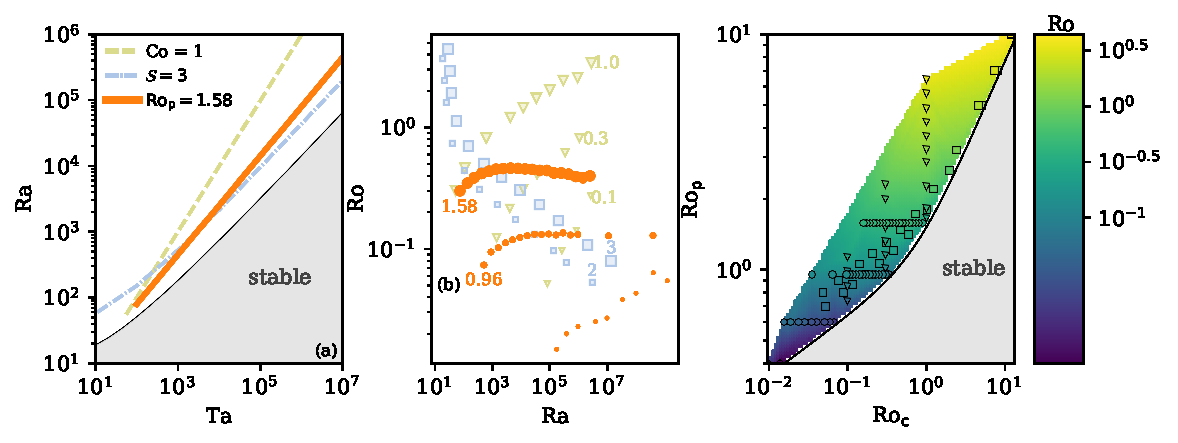
\includegraphics[width=\textwidth]{parameter_space.pdf}
    \caption{(a) The critical Rayleigh number, as a function of the Taylor number, 
    is plotted as a solid black line. The grey shaded region is subcritical, and rotation
    supresses convection there. Paths of constant Convective Rossby number
    ($\con$, green dashed line), constant supercriticality ($\mathcal{S}$, blue dash-dot line), and 
    constant Predictive Rossby number (\pro, orange solid line) are shown through parameter space. 
    (b) Evolved Ro is plotted vs. Ra along paths of \pro = [1.58, 0.96] for [big, small] orange circles.
    For comparison, paths of constant $\mathcal{S}$ (blue squares, $\mathcal{S} = [3,2]$ 
    for [big, small] squares)
    and constant $\con$ (green triangles, $\con$ = [1, 0.3, 0.1] for [big, medium, small] triangles) are shown.
    Ro is roughly constant for a constant \pro, particularly for the low-Ro, $\pro=0.96$ case, 
    but changes drastically at constant $\con$ or $\mathcal{S}$.
    (c) The evolved value of Ro is shown as a function of $\pro$ and $\con$. 
	Each of the experiments in (b) is outlined by a black (circle, triangle, square)
	for points along constant (\pro, \con, $\mathcal{S}$) paths.
	The color inside of the marker represents the exact measured Ro of that experiment, 
	while the colormap outside of markers is a linear interpolation
	of the data set. A least-squares fit to all experiments with $\mathcal{S} \geq 1.5$ and
	$\text{Ro} \geq 0.3$ returns $\text{Ro} = 0.2 \con^{-0.19}\pro^{1.5}$. A similar fit to all experiments with
	$\mathcal{S} \geq 1.5$ and $\text{Ro} < 0.3$ returns $\text{Ro} = 0.1 \con^{-0.21}\pro^{3.5}$. 
	In both the high- and low- Ro regime, the measured
	Rossby number is a strong function of $\pro$ and a weak function of $\con$.
    \label{fig:parameter_space} }
\end{figure*}


The critical value of Ra at which convection onsets also depends on Ta (see the black line in figure \ref{fig:parameter_space}a);  
roughly according to $\text{Ra}_{\text{crit}} \sim \text{Ta}^{2/3}$ \citep{Chandrasekhar,calkins&all2015a}.
We have confirmed these scalings of $\text{Ra}_{\text{crit}}(\text{Ta})$ and 
$k_{\text{crit}}(\text{Ta})$ in our atmospheres using a linear
stability analysis.
Even taking account of linear theory, the dependence of the evolved nonlinear fluid 
flows on the input parameters makes predicting the rotational constraint very challenging. 
We will explore three paths through Ra-Ta space:
\begin{equation}
    \text{Ra} = 
    \begin{cases}
    \mathcal{S}\,\text{Ra}_\text{crit}(\text{Ta}), & (\text{I})\\
    (\con)^2 \, \text{Pr}\, \text{Ta}, & (\text{II}) \\
    (\pro)^2\, \text{Pr}\, \text{Ta}^{3/4} & (\text{III}).
    \end{cases}
    \label{eqn:paths}
\end{equation}
Paths on constraint I are at constant supercriticality, 
$\mathcal{S} \equiv \text{Ra}/\text{Ra}_{\text{crit}}$
(blue dash-dot line in figure \ref{fig:parameter_space}a).
Paths on constraint II are at a constant value of the classic $\con$ (green dashed line in figure \ref{fig:parameter_space}a). Paths on constraint
III (e.g., orange solid line in figure \ref{fig:parameter_space}a) 
set constant a ratio which we call the ``Predictive Rossby number,'' 
\begin{equation}
\pro = \sqrt{\frac{\text{Ra}}{\text{Pr}\,\text{Ta}^{3/4}}} \ = \    
\frac{1}{(2 \Omega)^{3/4}} \sqrt{\frac{g \, \Delta  S}{c_{p} \nu^{1/2}}}
\end{equation}
To our knowledge, these paths have not been reported in the literature. 
Paths along constant \con$\,$are sensitive to the depth of the domain, 
but are blind to changes in diffusivities with increasing Ra and Ta. 
On the other hand, paths with constant \pro$\,$ 
feel changes in diffusivities but not the depth of the domain.

%The importance of the predictive Rossby number implies the importance of a 
%dynamical length scale, 
%\begin{equation}
%L_{\text{p}} \ \sim \ \frac{L_{z}}{\text{Ta}^{1/4}} \label{L-star}
%\end{equation}
%This differs noticeably from the anticipated onset length scale 
%\begin{equation}
%L_{\text{crit.}} \ \sim \ \frac{L_{z}}{\text{Ta}^{1/6}}.
%\end{equation}
%Length-scale corrections of the form of equation \ref{L-star} 
%have been proposed in systems with no-slip boundary conditions and Ekman pumping effects. However, we see this scale in a system with stress-free boundaries and ostensibly no significant Ekman fluxes. 

%%%%%%%%%%%%%%%%%%%%%%%%%%%%%%%%%%%%%%%%%%%%%%%%%%%%%%%%%%%%%%%%%%%%%%%%%%%%%%%
%% RESULTS SECTION
\section{Results}
\label{sec:results}
In figure~\ref{fig:parameter_space}a, the value of Ra$_{\text{crit}}$
is shown as a function of Ta, as
calculated by a linear instability analysis. A sample path for
each criterion in equation~\ref{eqn:paths} through
this parameter space is shown.
In figure \ref{fig:parameter_space}b, we display the evolution of Ro
with increasing Ra along various paths through parameter space.
We find that Ro increases on constant \con$\,$paths, decreases on constant $\mathcal{S}$
paths, and remains roughly constant along constant \pro$\,$ paths.
In figure \ref{fig:parameter_space}c, the value of Ro is shown simultaneously as
a function of \pro$\,$and \con$\,$for all experiments conducted in this study.
We find a general power-law of the form \mbox{$\text{Ro} \propto \con^{-1/5}\,\pro^{\alpha}$},
where $\alpha \approx 3.5$ in the rotationally constrained, low-Ro regime and
\mbox{$\alpha \approx 1.5$} in the unconstrained, high-Ro regime. 
In the rotationally constrained regime, Ro is a much stronger function of 
$\pro\,$than $\con$, and the
evolved Ro can be approximately determined through specification of \pro$\,$alone.


%%%%%%%%%%%%%%%%%%%%%%%%%%%%%%%%%%%%%%%%%%%%%%%%%%%%%%%%%%%%%%%%%%%%%%%%%%%%%%%
%% DYNAMICS FIGURE
\begin{figure*}[t]
    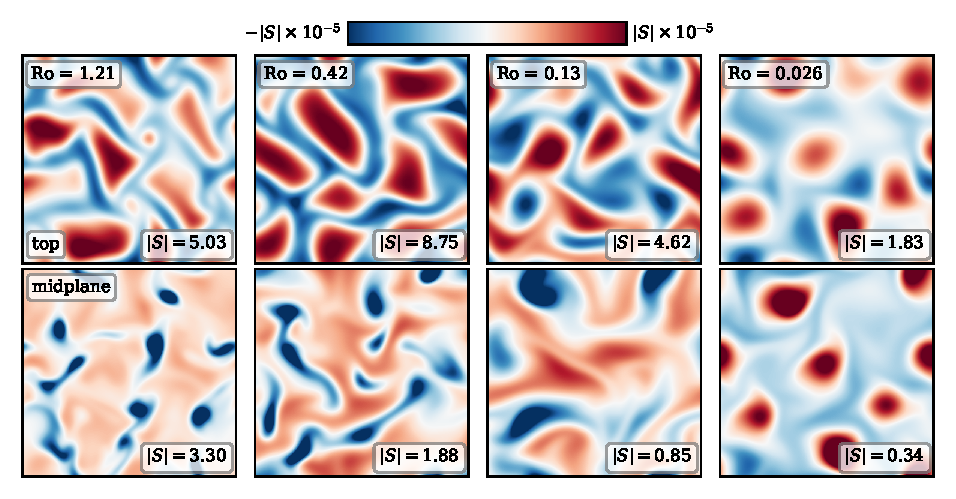
\includegraphics[width=\textwidth]{dynamics_plot.pdf}
    \caption{ A horizontal slice of the evolved entropy field is plotted at $z = 0.95L_z$
    for select simulations. The mean value of entropy at this height has been removed in all
    cases. All runs displayed here have an evolved volume-averaged $\text{Re} \approx 200$. 
    As Ro decreases from O(1) on the left to O(0.1) on the right, and thus the rotational
    constraint on the flow increases, significant changes in flow morphology are observed.
    At Ro = 2.01 ($\con = 1$), convective dynamics are not hugely dissimilar from the non-rotating
    case where there are large upflows and narrow, fast downflow lanes (see e.g., \AB).
    As the rotational constraint increases, the granular convective pattern gives way
    to vortical columns, as seen at Ro = 0.13 ($\pro = 0.96$).
    \label{fig:pretty_convection} }
\end{figure*}

%%%%%%%%%%%%%%%%%%%%%%%%%%%%%%%%%%%%%%%%%%%%%%%%%%%%%%%%%%%%%%%%%%%%%%%%%%%%%%%
%% NU AND RE FIGURE
\begin{figure}[t!]
    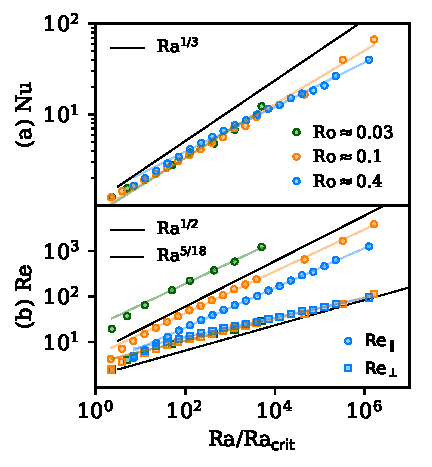
\includegraphics{nu_and_re.pdf}
    \caption{Scaling laws for paths at $\pro = 1.58$ ($\text{Ro} \approx 0.4$) and
    $\pro = 0.96$ ($\text{Ro} \approx 0.1$) are shown. 
    (a) Evolved Nu vs. Ra. The scaling laws here are very reminiscent of classic \RB convection
    theory \citep{ahlers&all2009}.
    (b) Evolved Re vs. Ra.
    The scaling seen here is nearly identical to scalings in nonrotating convection (\AB).
    \label{fig:nu_and_re} }
\end{figure}

%%%%%%%%%%%%%%%%%%%%%%%%%%%%%%%%%%%%%%%%%%%%%%%%%%%%%%%%%%%%%%%%%%%%%%%%%%%%%%
%% BOUNDARY LAYER FIGURE
\begin{figure*}[ht!]
    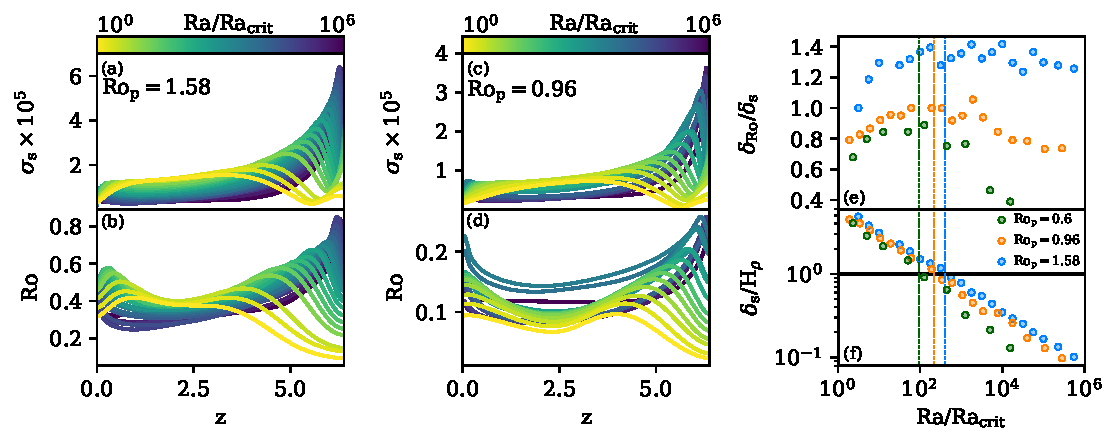
\includegraphics[width=\textwidth]{boundary_layers.pdf}
    \caption{Horizontally-averaged profiles of the $z$-derivative of 
    the specific entropy profile ($\partial_z s$, a) and Rossby number (Ro, b) 
    are shown vs. height for $\pro = 0.96$ ($\text{Ro} \approx 0.1$). 
    Similar profiles are shown in (c) and (d) for $\pro = 1.58$ ($\text{Ro} \approx 0.4$). The color of the profiles
    denotes the value of Ra, with yellow profiles being at very low Ra and purple at the highest
    values of Ra studied here.
    (e) The ratio of the thicknesses of the dynamical (Ro) boundary layers and 
    thermal ($\partial_z s$) boundary layers is shown for both values of \pro$\,$at each value of Ra.
    This ratio, and thus the relative importance of both thermal and rotational dynamics,
	remains roughly constant across orders of magnitude of Ra.
    \label{fig:profiles_and_bls} }
\end{figure*}

In figure~\ref{fig:pretty_convection}, sample snapshots
of the evolved entropy field in the $x$-$y$ plane near the top of the domain are shown. 
In the left panel is a rotationally unconstrained flow at moderately high
Ro, and Ro decreases into the rotationally constrained regime from left to right.
As Ro decreases, the
classic granular structure of convection (see e.g., figure~2 in \AB) gives way to vortical
columns of convection, as seen in rapidly rotating \RB convection \citep{stellmach&all2014}.
The select cases displayed in figure~\ref{fig:pretty_convection} each have an evolved volume-averaged
$\text{Re} \approx 200$.

We measure the Nusselt number (Nu), which quantifies heat transport in a convective
solution, as defined in \AB.
In figure~\ref{fig:nu_and_re}a, we show how Nu scales as a function
of Ra at fixed \pro. When $\text{Ro} \approx 0.1$,
we find a scaling of $\text{Nu} \propto \text{Ra}^{0.27}$. This is reminiscent of
classic scaling laws (e.g., Ra$^{2/7}$) in non-rotating \RB convection \citep{ahlers&all2009}.
This suggests that changes in heat transport at constant \pro$\,$are driven by
changes in the thermal boundary layer structure with increasing Ra.
In figure \ref{fig:nu_and_re}b, we plot the RMS Reynold's
number (Re $= |u| L_z / \nu$) as a function of Ra at fixed \pro, and find that 
$\text{Re} \propto \text{Ra}^{0.47}$ in the rotationally constrained regime,
which is almost precisely the $\text{Re} \propto \text{Ra}^{1/2}$ scaling measured
in the non-rotating regime in \AB.

Figure \ref{fig:profiles_and_bls} shows time- and horizontally-averaged profiles of
Ro and the z-component of the specific entropy gradient, $\partial_z s$.
Figures \ref{fig:profiles_and_bls}a\&b show these profiles for $\pro=0.96$ ($\text{Ro} \approx 0.1$), while
Figures \ref{fig:profiles_and_bls}c\&d show these profiles for $\pro=1.58$ ($\text{Ro} \approx 0.4$). The transition
in profile behavior from low Ra (yellow) to high Ra (purple) is denoted by the color of the
profile.
As Ra increases at a constant value of
\pro, both the thermal ($\partial_z s$) and dynamical (Ro) boundary layers become thinner. 
We measure the
thickness of the thermal boundary layer ($\delta_{s}$) at the top of the domain by 
measuring where a linear fit within the boundary layer crosses through $\partial_z s = 0$.
We ensure by-eye for each profile that this is a reasonable measure of the boundary
layer thickness. We measure
the thickness of the Ro boundary layer ($\delta_{\text{Ro}}$) 
as the height of the peak value of Ro within the
upper half of the domain.
In figure \ref{fig:profiles_and_bls}e, we plot $\delta_{\text{Ro}}/\delta_{s}$, the ratio
of the sizes of these two boundary layers. As anticipated, the dynamical boundary layer ($\delta_{\text{Ro}}$)
becomes relatively thinner with respect to the thermal boundary layer ($\delta_{s}$)
as Ro and \pro$\,$ decrease. At $\pro = 1.58$, both boundary layers are approximately equally
thick, and so both rotational and advective effects are equally important. On the other hand,
at $\pro = 0.96$, the dynamical boundary layer is only 60\% the size of the thermal boundary
layer, and rotational effects dominate the dynamics.

%%%%%%%%%%%%%%%%%%%%%%%%%%%%%%%%%%%%%%%%%%%%%%%%%%%%%%%%%%%%%%%%%%%%%%%%%%%%%%%
%% CONCLUSION SECTION
\section{Discussion}
\label{sec:discussion}
In this letter, we studied low-Mach-number, stratified, compressible convection 
under the influence of rotation.
We examined three paths through Ra-Ta space, and showed that in the rotationally
constrained regime at low-Ro, the newly-defined 
Predictive Rossby number, $\pro = \text{Ra}/(\text{Pr }\text{Ta}^{3/4})$, determines the value of
the evolved Ro. While increasing Ra and holding \pro$\,$ constant,
we find scaling laws of heat transport (Nu) and turbulence (Re) that are nearly identical
to scaling laws seen in nonrotational convection.
We note briefly that the scaling $\text{Ra} \propto \text{Ta}^{3/4}$ is very similar to
the theorized boundary between fully rotationally constrained convection and 
partially constrained convection predicted in Boussinesq theory, of 
$\text{Ra} \propto \text{Ta}^{4/5}$ \citep{julien&all2012, gastine&all2016}. This
Ta$^{4/5}$ scaling arises through arguments of geostrophic balance in the boundary layers,
and is a steeper scaling than the Ta$^{3/4}$ scaling present in \pro.
This suggests that at sufficiently low \pro, a suite of simulations across many orders
of magnitude of Ra will not only have the same volume-averaged value of Ro 
(as in Fig.~\ref{fig:parameter_space}b), but will
also maintain proper force balances within the boundary layers.

Our results suggest that by choosing the proper value of \pro, experimenters
can select the degree of rotational constraint present in their simulations. 
Once that value is chosen, it is straightforward to increase the turbulent nature of 
the simulations by increasing Ra, just as in the non-rotating case.
Although all the results reported here are for a Cartesian geometry with 
antiparallel gravity and rotation, preliminary 3D spherical simulations suggest that 
\pro$\,$ also specifies Ro in more complex geometries (Brown et al. 2019 in prep).


\begin{acknowledgements}
This work was supported by NASA Headquarters under the NASA Earth and Space
Science Fellowship Program -- Grant 80NSSC18K1199.
EHA further acknowledges the University of Colorado's George 
Ellery Hale Graduate Student Fellowship.
This work was additionally supported by  NASA LWS grant number NNX16AC92G.  
Computations were conducted 
with support by the NASA High End Computing (HEC) Program through the NASA 
Advanced Supercomputing (NAS) Division at Ames Research Center on Pleiades
with allocation GID s1647.
\end{acknowledgements}

\bibliography{biblio.bib}
\end{document}
